\chapter{Introduction}

This chapter will introduce the notion of rephotography, elaborate on the
process of how to make such a photograph and evaluate existing approaches to
simplify it. These include two applications for mobile operating systems which
will be briefly discussed. Furthermore, a summary of more sophisticated work by
MIT researchers will be given, leading to the problem statement and the goal of
this work.

\section{Overview}

Rephotography or repeat photography denotes the retrieval of the precise viewpoint used for taking a
--- possibly historic --- photograph and capturing another image from the same
spot, ideally with the same camera parameters. This allows for documentation and
visualisation of changes which the scene has undergone between the two or more
captures.  For instance when documenting urban development, one can present
progress of construction, restoration efforts or changes in the surroundings in
a visually striking manner, e.g. by blending the photographs together.
Figures \autoref{fig1} and \autoref{fig2} show examples.

\begin{figure}
   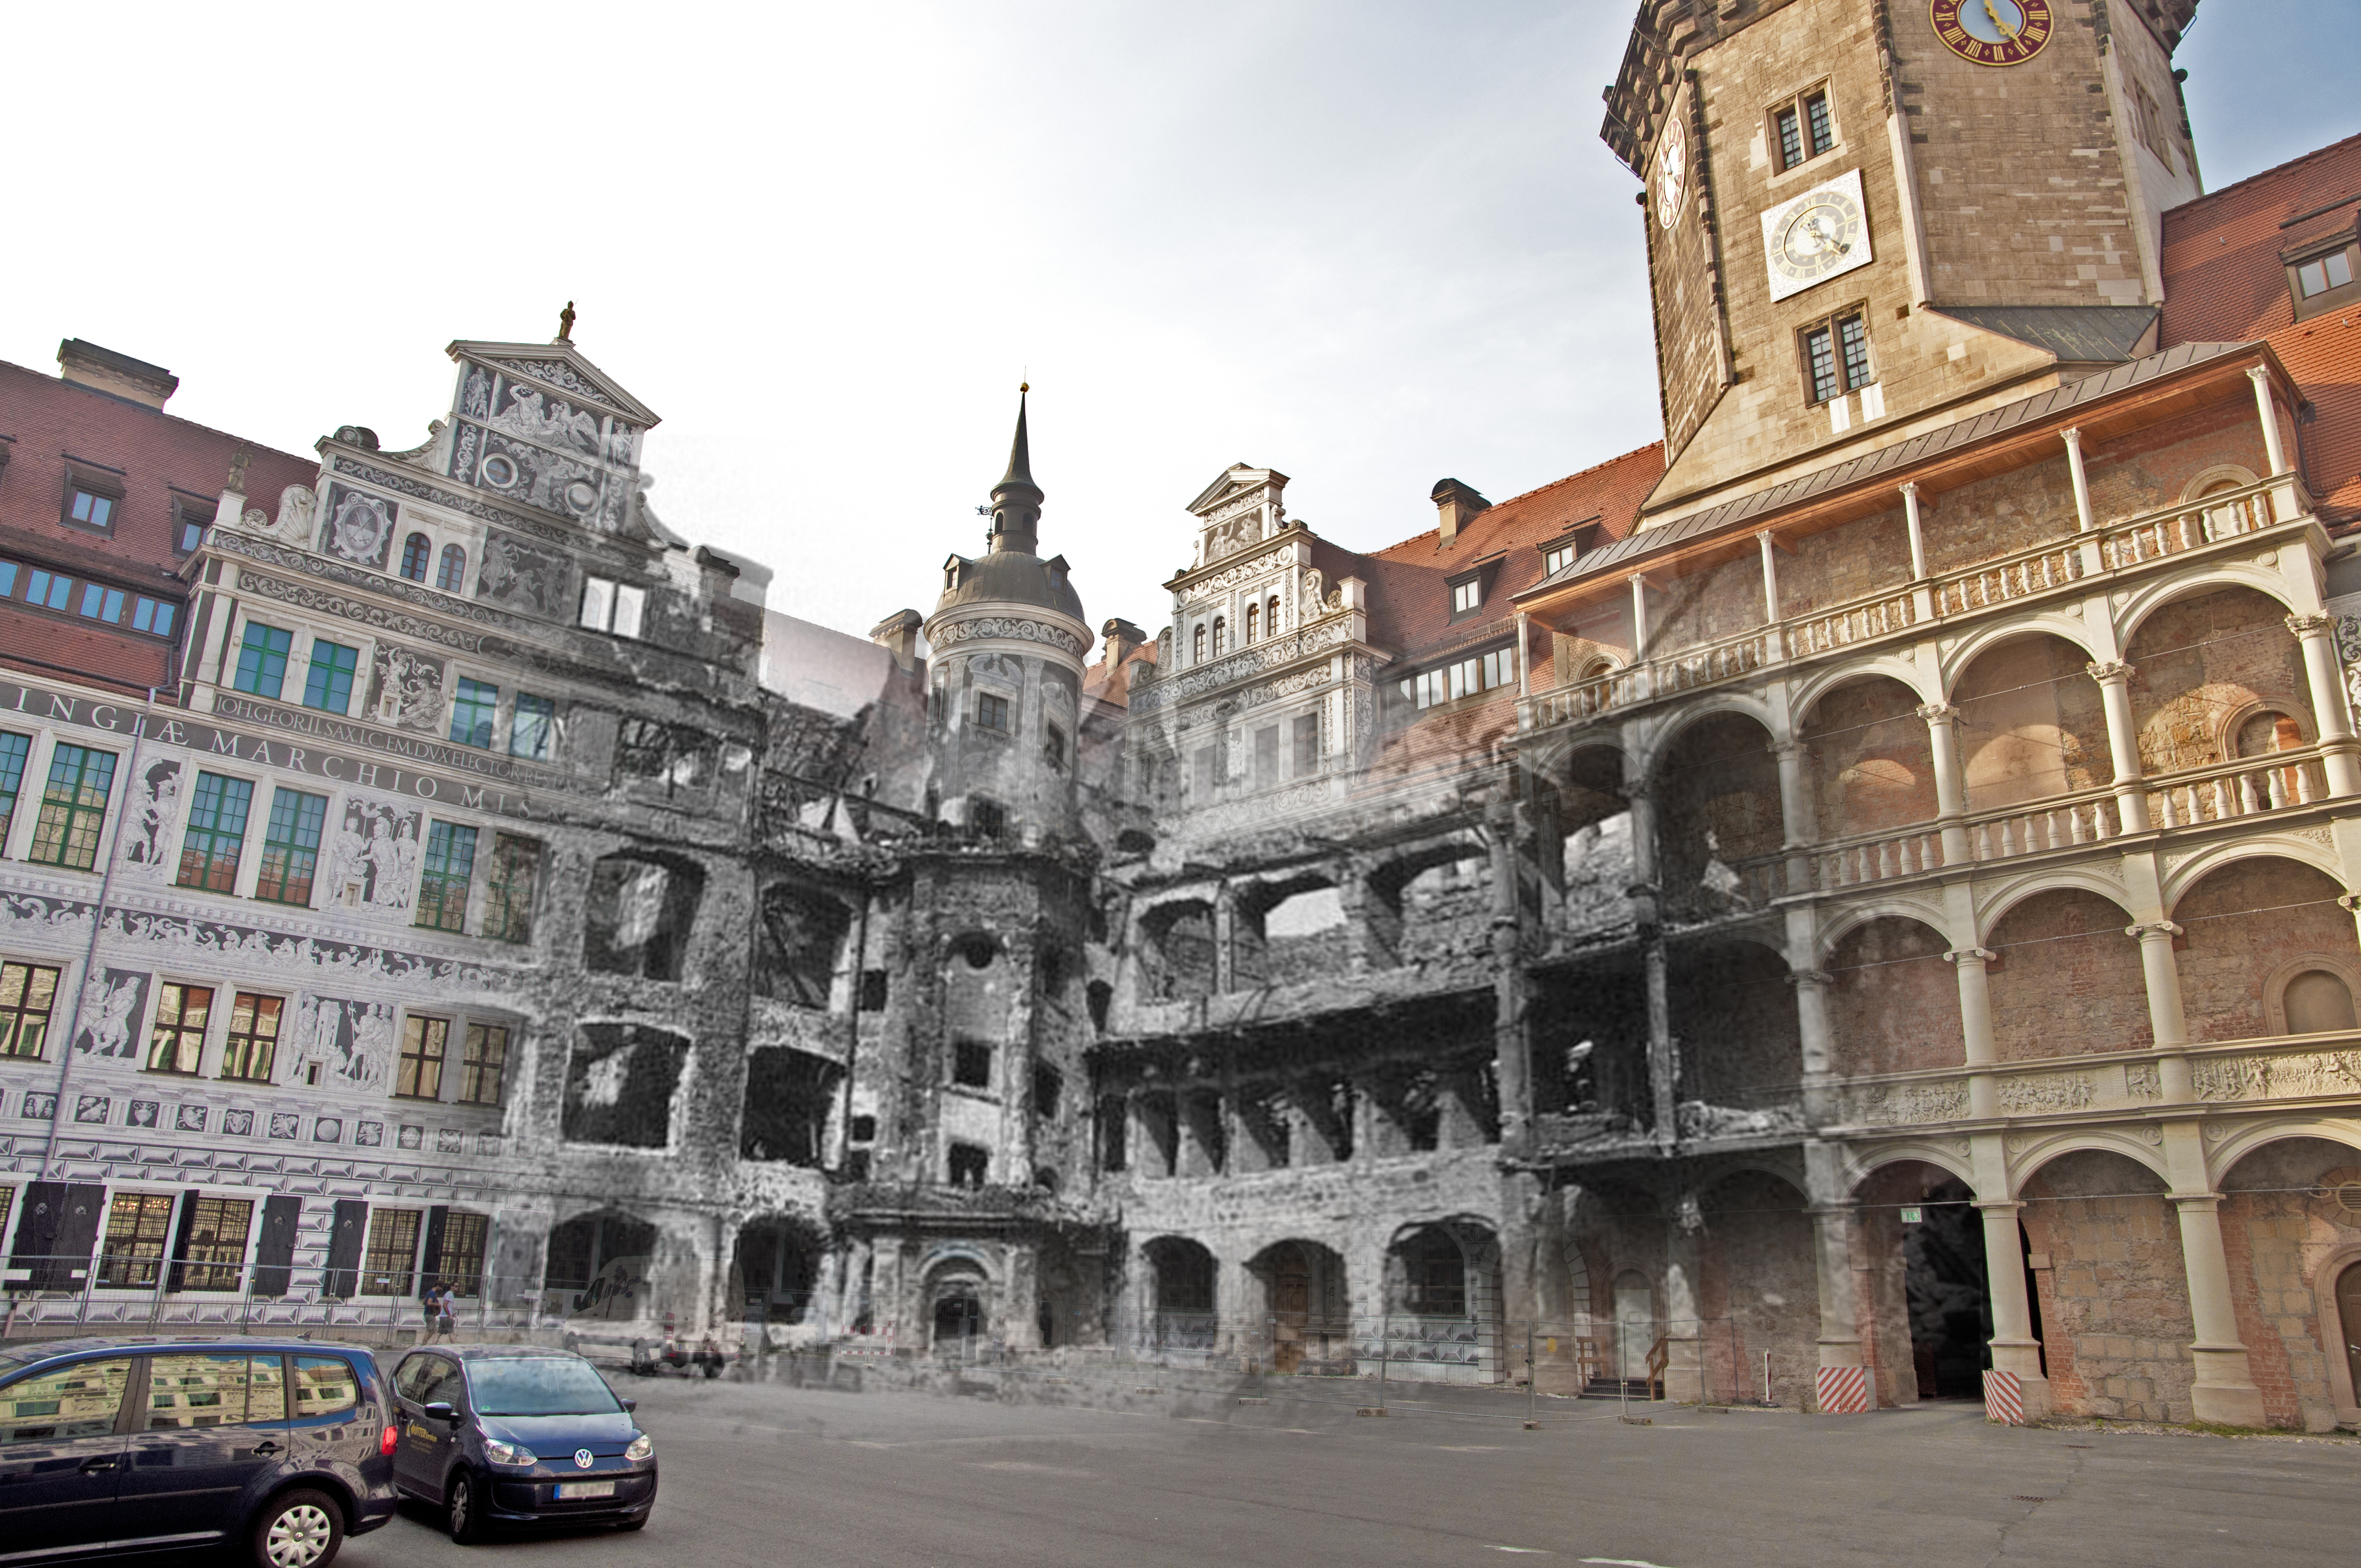
\includegraphics[width=\textwidth]{gfx/1945_2014_Residenzschloss.jpg}
   \caption{Residenzschloss Dresden, destroyed during World War II,
   \textcopyright\ Sergey Larenkov, printed with permission}
   \label{fig1}
\end{figure}

\begin{figure}
   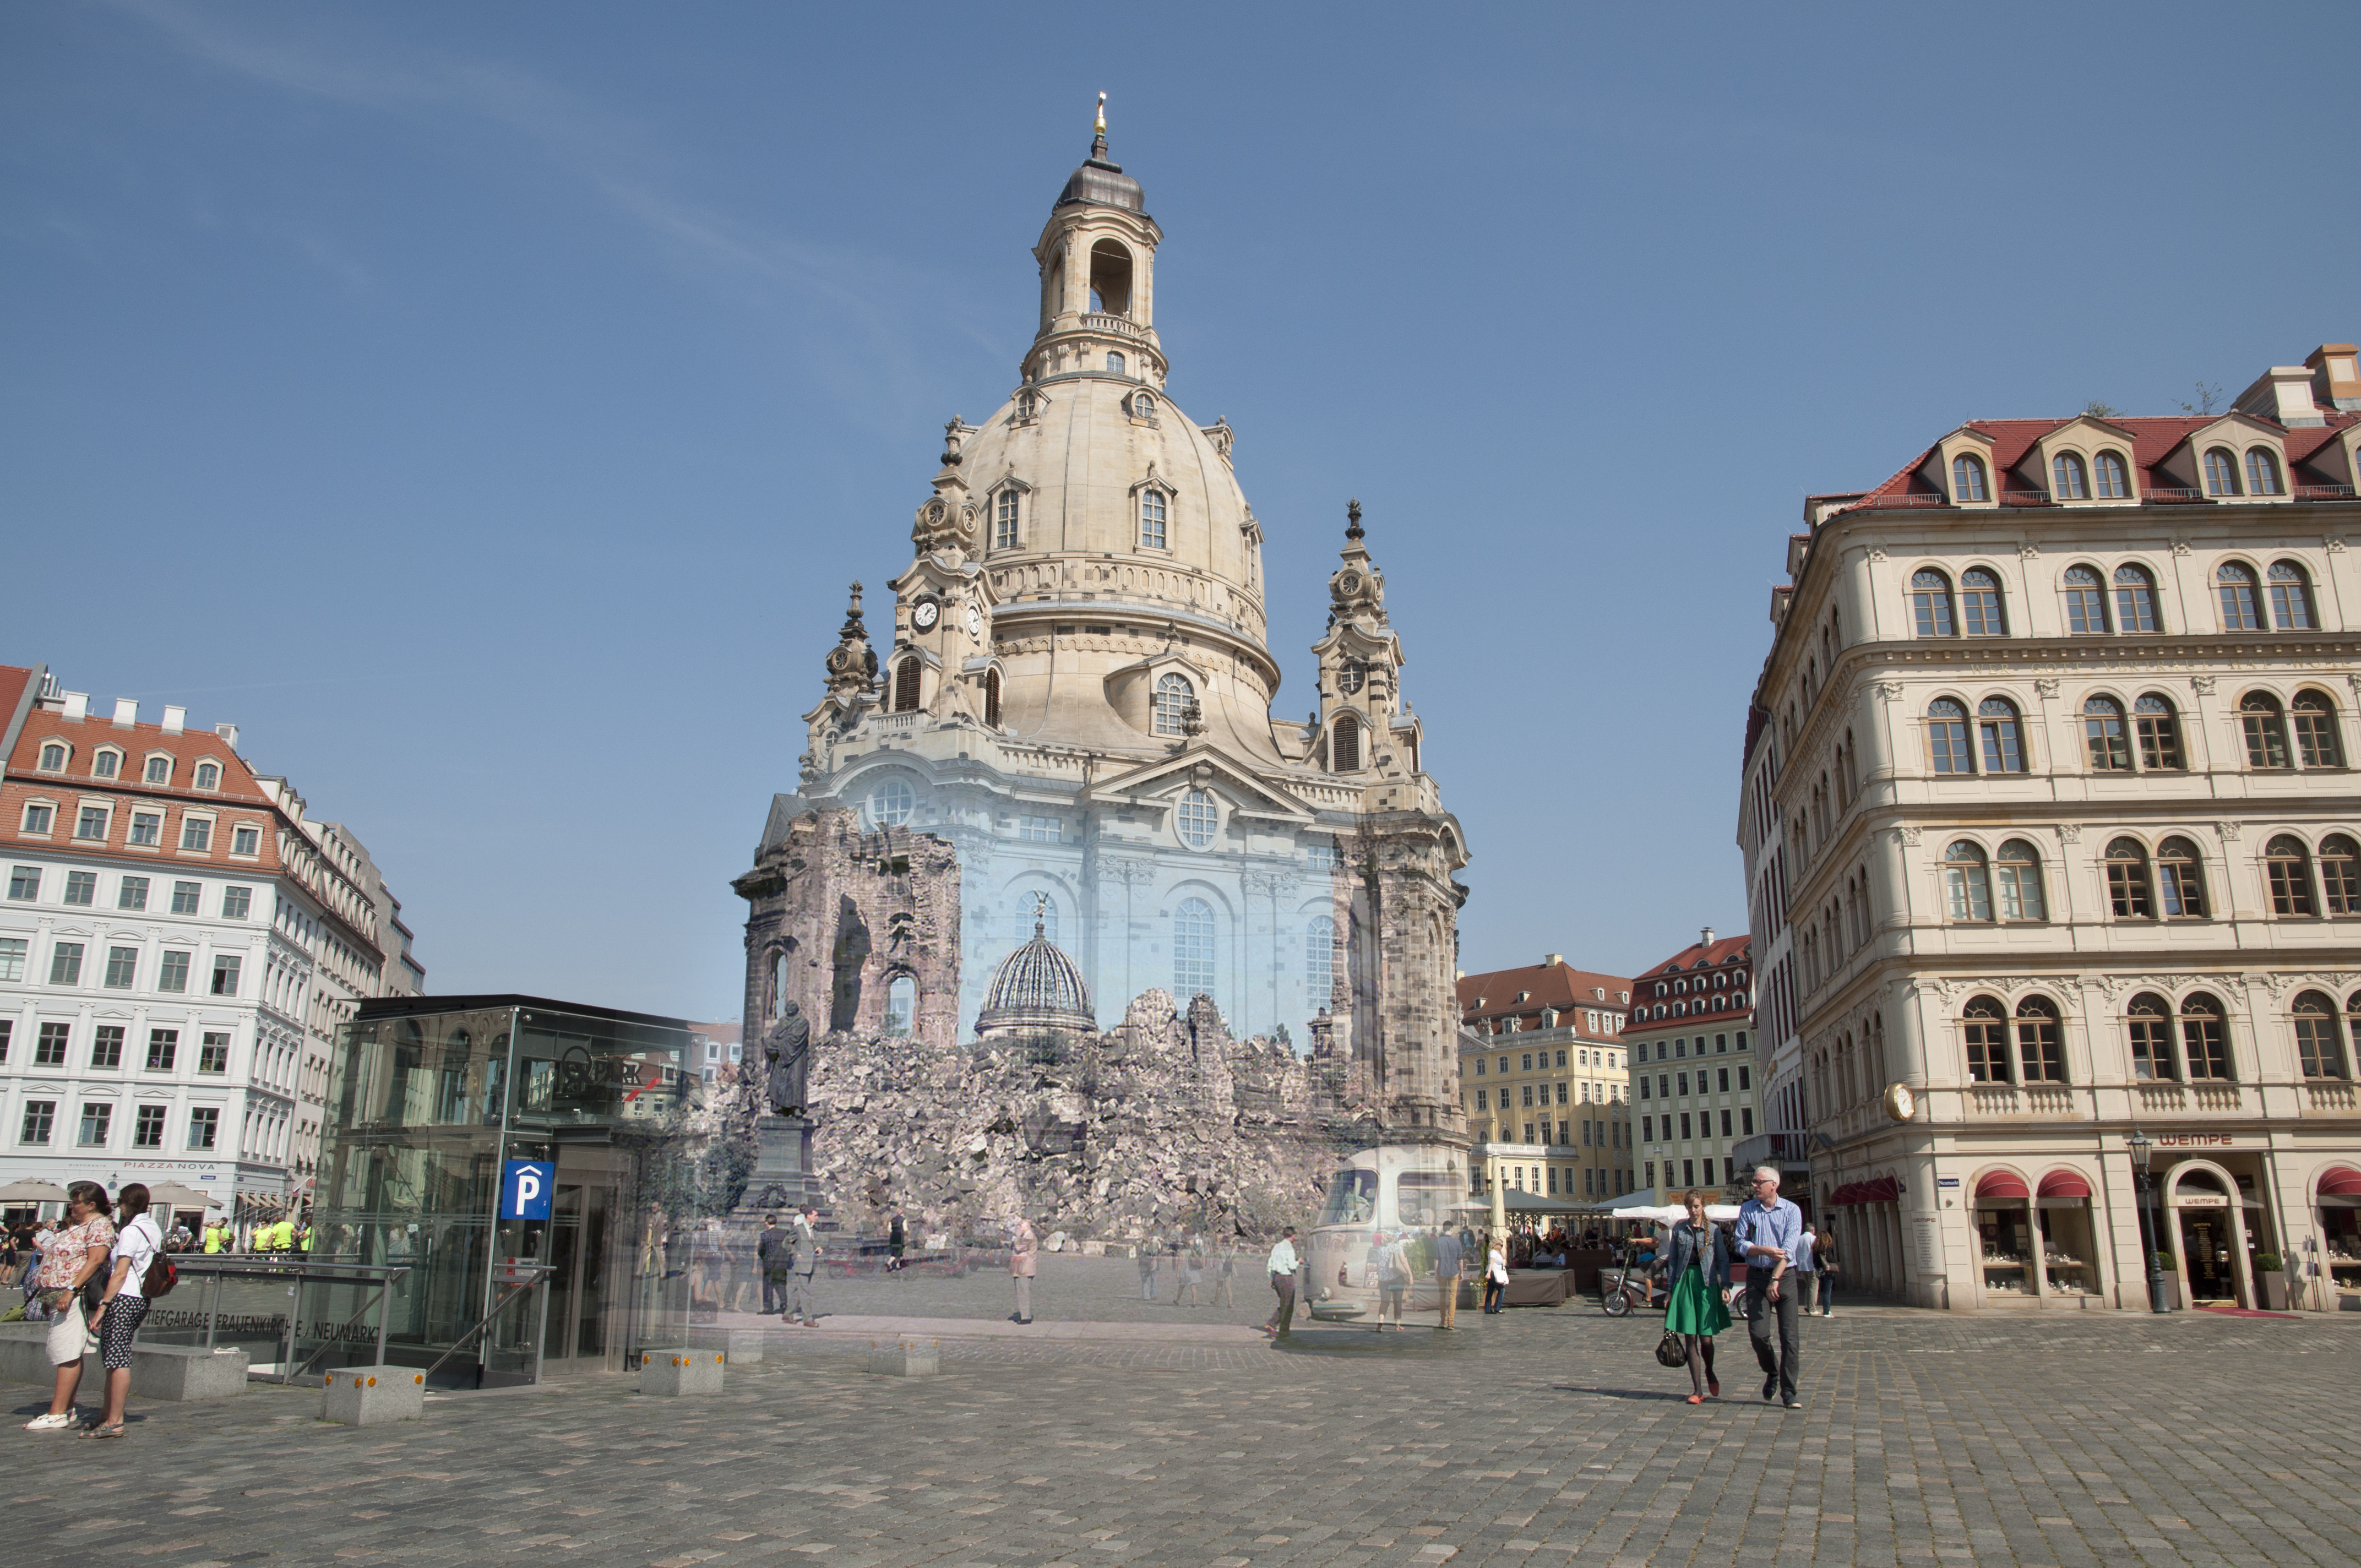
\includegraphics[width=\textwidth]{gfx/1950_2014_Frauenkirche.jpg}
   \caption{Frauenkirche Dresden, destroyed during World War II,
   \textcopyright\ Sergey Larenkov, printed with permission}
   \label{fig2}
\end{figure}

When done manually, the photographer must attempt to find the original viewpoint 
usually by visual inspection of the original image and trying to match the
current camera parameters --- camera position, camera rotation, focal length,
possibly principal point --- to the original.
The procedure is often carried out by placing the camera on a tripod and
comparing a printout of the original image with what can be seen through the
viewfinder or the camera screen. The number of parameters to match as well as
the difficulty to estimate them purely from comparing two-dimensional images makes the process
error-prone and tedious. Visual acuity and experience of the photographer thus
place limits on the accuracy with which the camera pose of the reference image
can be reconstructed. Some corrections can be done by post-processing the images
and warping the rephotograph with a homography to better match the original.

At the time of writing, few computerized aids are available to the
photographer (see below).
The advancement of mobile phones and tablet computers with integrated cameras
and larger screens presents the opportunity to develop applications which can
assist in this endeavour, moving away from the traditional trial-and-error
approach.  On current digital cameras\footnote{At the time of writing, no
   commercial manufacturer produces a camera with user-modifiable firm- or
software. A project at Stanford \citep{Levoy2010} was discontinued
\cite{FrankenCam}} this is impossible due to their closed infrastructure not
permitting running user programs. 

\section{Previous Approaches}

\subsection{Mobile Applications}

Two applications have been developed to assist a photographer in taking
rephotographs. For smartphone operating systems,
\emph{rePhoto}\footnote{\url{http://projectrephoto.com/}} and
\emph{Timera}\footnote{\url{http://www.timera.com/Explore}} exist, both
available for Android and iOS devices. These applications support the user by placing a transparent
version of the original image over the current camera image, allowing for easier
alignment. The captured rephotograph is then presented together with the
original image in a blend (c.f. \autoref{fig3}) which can be customized in
\emph{Timera}.

What is characteristical about both of these applications is that the user must still
determine on their own how to actually move the camera. An overlay simplifies
the procedure, eliminating some of the inaccuracy introduced into the manual approach by the
necessity to move the eyes from printout to camera, but it is still the user's
responsibility to determine the necessary motion between the current camera
position and the goal position (that of the original image). 


\subsection{Computational Re-Photography}

A more
sophisticated automated approach was presented in \citep{bae2010} by MIT researchers in
2010. In this setup, the relevant parameters of a historic image's camera are
reconstructed, including the focal length, principal point and the six degrees
of freedom in camera pose and after reconstructing the scenery in 3D by use of
two images captured by the user, they are then directed by the software to the
desired viewpoint.

Bae et. al identify five primary obstacles in viewpoint reconstruction of a
historic photograph
\begin{enumerate}
   \item The necessary camera motion has six degrees of freedom --- three for
      translation and three for rotation --- which are challenging for the user
      to adjust simultaneously, as changing one parameter will often necessitate
      adjustments for the others to improve the matching. Furthermore, the
      number of degrees of freedom makes it difficult to communicate to the
      user, how they must move the camera.
   \item 3D reconstruction is possible only up to an unknown scale (see
      \autoref{section on projective geometry}), meaning it is impossible to
      determine e.g. if an object viewed by the camera is small and close or
      large and further away. This poses the problem of how to determine if the
      user is close to the desired viewpoint and whether or not they have come
      closer or moved further away over iterations. 
   \item Relative pose estimation from corresponding points fails when the
      motion between the two cameras approaches zero, which is the ultimate goal
      one wishes to achieve. When na\"ivley comparing the current camera image
      to the reference photograph, the estimate for relative rotation and
      translation becomes increasingly unreliable as the camera approaches the
      original viewpoint.
   \item Automated computation of relative camera pose will rely on feature
      detection to find correspondences. However, historical images will often
      be vastly different from the current scene. Not only may the scene itself
      have changed considerably, but also the historical image --- having been
      taken by a historical camera --- may differ in contrast, sharpness and
      colours. Feature detectors may not be able to reliably find
      correspondences when comparing an old with a new photograph.
   \item The calibration data --- most importantly, focal length and principal
      point --- of the historical camera are often unknown. The calibration data
      is needed for relative pose computation.
\end{enumerate}


